%----------------------------------------------------------------------------------------
%   PACKAGES AND DOCUMENT CONFIGURATIONS
%----------------------------------------------------------------------------------------

\documentclass[12pt]{article}
\usepackage[english]{babel}
\usepackage[utf8]{inputenc}
\usepackage{float}

\usepackage{graphicx,epstopdf}   %for embedding images and for conveting eps to pdf
\usepackage{subfig}              %for sub images
\usepackage[margin=1in,includefoot]{geometry}	%changes the margins of report to 1 in
\usepackage{lscape}

\usepackage{rotating}   %used for rotating figures
\usepackage[automake,nonumberlist]{glossaries}    %To use glossary
\usepackage{varwidth}
\usepackage{multicol}   %for making columns
\usepackage{amsmath}
\usepackage{appendix}
\usepackage{pdfpages}
\usepackage{empheq}
\usepackage{hyperref}
\usepackage{xcolor}
\usepackage{rotating}

\usepackage[framed, numbered]{matlab-prettifier}    %to import matlab code

%----------------------------------------------------------------------------------------
%   Acronym/Glossary
%----------------------------------------------------------------------------------------
\makeglossaries
\loadglsentries{glossary}

%----------------------------------------------------------------------------------------
%   Document Start
%----------------------------------------------------------------------------------------

\begin{document}

\begin{titlepage}

\newcommand{\HRule}{\rule{\linewidth}{0.5mm}} % Defines a new command for the horizontal lines, change thickness here

\center % Center everything on the page
 
%----------------------------------------------------------------------------------------
%   HEADING SECTIONS
%----------------------------------------------------------------------------------------

\textsc{\LARGE MSE 211 Computational Methods for Engineers}\\[1.5cm] % Org Name
\textsc{\Large }\\[0.5cm] % course name
\textsc{\large }\\[0.5cm] % course title

%----------------------------------------------------------------------------------------
%   TITLE SECTION
%----------------------------------------------------------------------------------------

\HRule \\[0.4cm]
{ \huge \bfseries Lab 2: Optimization}\\[0.4cm] % Title of report
\HRule \\[1.5cm]
 
%----------------------------------------------------------------------------------------
%   AUTHOR SECTION
%----------------------------------------------------------------------------------------

\begin{minipage}{0.4\textwidth}
    \begin{flushleft} \large
        \emph{Authors:}\\
        Parshant \textsc{Bombhi}\\
        Shivam \textsc{Bhardwaj}\\
        Aidan \textsc{Hunter}\\
        Ataur \textsc{Rehman}
    \end{flushleft}
\end{minipage}
\hfill
\begin{minipage}{0.4\textwidth}
    \begin{flushright} \large
        \emph{Student ID:} \\
        301255126\\
        301302118\\
        301279938\\
        301253848
    \end{flushright}
\end{minipage}
\vspace{10mm}
%----------------------------------------------------------------------------------------
%   DATE SECTION
%----------------------------------------------------------------------------------------

{\large \today}\\[2cm] % Date, change the \today to a set date if you want to be precise

%----------------------------------------------------------------------------------------
%   LOGO SECTION
%----------------------------------------------------------------------------------------

\includegraphics[scale=2.0]{MSE-Logo.jpg}\\[1cm] %logo
%----------------------------------------------------------------------------------------

\vfill % Fill the rest of the page with whitespace

\end{titlepage}

%----------------------------------------------------------------------------------------
%   Table of Contents/Table of Figures
%----------------------------------------------------------------------------------------
\pagenumbering{roman} %sets numbering of page to roman
\tableofcontents	%makes table of contents
\addcontentsline{toc}{section}{\numberline{}Table Of Contents}	%adds TOC to TOC

\listoffigures
\addcontentsline{toc}{section}{\numberline{}List of Figures}	%adds list of figures to table of contents

 \listoftables
 \addcontentsline{toc}{section}{\numberline{}List of Tables}

\lstlistoflistings
\addcontentsline{toc}{section}{\numberline{}Listings}

% \printglossary
% \addcontentsline{toc}{section}{\numberline{}Glossary}	%adds glossary to table of contents
\pagebreak
%----------------------------------------------------------------------------------------
%   Main Body
%----------------------------------------------------------------------------------------
\setcounter{page}{1}	%resets the page numbering
\pagenumbering{arabic}	%sets numbering of page to arabic
\setlength{\parskip}{1em}

\section{Introduction}

\section{Methodology}
\subsection{Comparison of Optimization Methods}
\subsubsection{Steepest Descent Method}
As per the lab manual, the steepest descent method consists of starting a initial point and the direction of the steepest descent is determined, using the gradient. Then with a calculated step size the algorithm progress towards the minimum. In two dimension  the solution is rather trivial, however, the function to be minimized is in 3D dimension. Therefore, the general format of the steepest descent method is described below.

To calculate the step size, the Hessian and the gradient are used: 
\begin{align}
  \textbf{H(x)}_{ij} &\equiv  
  \begin{bmatrix}
    \dfrac{\partial^2 f}{\partial x^2} & \dfrac{\partial^2 f}{\partial x \partial y} \\[2em]
    \dfrac{\partial^2 f}{\partial x \partial y} & \dfrac{\partial^2 f}{\partial y^2}
  \end{bmatrix}
\end{align}
The Hessian is an  calculated using the second partial derivative of the provided function as shown in equation \ref{eq:hess}
\begin{align}\label{eq:hess}
  \textbf{H(f)} &= 
  \begin{bmatrix}
    12x^2+4y-42 & 4x+4y \\[2em]
    4x+4y & 12y^2+4x-26
  \end{bmatrix}    
\end{align}
The gradient is calculated using the derivative of the provided function.
\begin{align}
\nabla(\textbf x) \equiv 
\begin{bmatrix}
\dfrac{\partial f}{\partial x}\\[2em]
\dfrac{\partial f}{\partial y}
\end{bmatrix}
\end{align}
Which gives us the gradient as shown in equation \ref{eq:grad} 
\begin{align}\label{eq:grad}
\nabla(f) =
\begin{bmatrix}
2x + 4x(x^2 + y - 11) + 2y^2 - 14\\[2em]
2y + 4y(y^2 + x - 7) + 2x^2 - 22
\end{bmatrix}
\end{align}
By using the hessian and the gradient we can calculate the step size for the method.
\begin{align}
    h= \left|  \frac{\nabla(x)^T \nabla(x)}{\nabla(x)^T H(x) \nabla(x)} \right|
\end{align}
The next iterations of x is based on current value minus the step size multiplied by gradient.
\begin{align}
    x_{i+1}=x_i-\nabla(x)h
\end{align}
Currently, the x will tend toward the minimum value , however if the - is changed to  + , the solution will tend toward the maximum value.

The aforementioned are used in a recursive manner to obtain the minimums value of the provided function. Essentially, the gradient, hessian, step size, and current x are recalculated in each iteration until the error between the new and current x are within 10E-6. 

\subsubsection{Newton's Method}
The Newton’s Method follows the same structure as steepest descent method, however the step size is modified, particularity  the step size is the inverse Hessian multiplied by gradient.
\begin{align}
    x_{i+1}=x_i-\textbf{H}^{-1}\nabla f(x_i)
\end{align}

\subsubsection{Matlab's Function}
In Matlab the function \textit{fminuc} is used to calculate the minimum values of the provided function, it also uses a recursive method to solve the for the minimum.\footnote{https://www.mathworks.com/help/optim/ug/fminunc.html}

It provides the options of quasi-newton or trust region, for the report the trust region was used. 
The trust region uses the quadratic method, the main equation is provide below. 
\pagebreak
\subsection{Synthesis of Mechanisms}
\subsubsection{Motion Generation}
\subsubsection{Path Generation}
Matlab was used to find the optimal dimensions and configuration of a 4-bar system acting as a walking spider, where the tip of the leg must pass through four precision points as a function of the input angle, a diagram of these points can be seen in figure \ref{fig:precionpoints_PG}.

\begin{figure}[h!]
    \centering
    \includegraphics[width=0.7\textwidth]{path_generation.png}
    \caption{Precision Point for Path Generation}
    \label{fig:precionpoints_PG}
\end{figure}
To find the optimal dimensions, a system of loop equations of the vector representations of the bars and relative angles between them were assembled and placed into a objective function to be minimized by a minimizing function in Matlab. This method was performed from the left and right side, shown in the figures below are the general structure of the left side analysis loop equations and the objective function, the red text are the unknown variables.
\begin{align}
    f_{jx}&=\color{red}r_{2x}\color{black}+\color{red}r'_{3x}\color{black}+\color{blue}\delta_{jx}\color{black}-\color{red}r'_{3x}\color{black}cos(\color{red}\alpha_j\color{black})+\color{red}r'_{3y}\color{black}sin(\color{red}\alpha_j\color{black})-\color{red}r_{2x}\color{black}cos(\color{blue}\beta_j\color{black})+\color{red}r_{2y}\color{black}sin(\color{blue}\beta_j\color{black})=0\\
    f_{jy}&=\color{red}r_{2y}\color{black}+\color{red}r'_{3y}\color{black}+\color{blue}\delta_{jy}\color{black}-\color{red}r'_{3y}\color{black}cos(\color{red}\alpha_j\color{black})+\color{red}r'_{3x}\color{black}sin(\color{red}\alpha_j\color{black})-\color{red}r_{2y}\color{black}cos(\color{blue}\beta_j\color{black})+\color{red}r_{2x}\color{black}sin(\color{blue}\beta_j\color{black})=0\\
    F&=\sqrt{(f_{1x})^2+f_{1y})^2+f_{2x})^2+f_{2y})^2+f_{3x})^2+f_{3y})^2}
\end{align}
\subsubsection{Function Generation}
The function generation method allows a continuous output based on input, primarily the input and output angles are known, and the required movement of the mechanism are to be calculated. For the purpose of this lab the movement of joint are specified, the input must travel 60 degrees and the output travels at 90 degrees.
\begin{figure}[h!]
    \centering
    \includegraphics[width=0.7\textwidth]{func_gen.png}
    \caption{Precision Point for Function Generation}
    \label{fig:precisionpoint_FG}
\end{figure}
The equation associated with each of the linkage movements are defined but the j is varied in the code.
\begin{multline}
    f_{jx}=-\color{blue}r_{2x}\color{black}cos(\color{blue}\beta_j\color{black})+\color{blue}r_{2y}\color{black}sin(\color{blue}\beta_j\color{black})-\color{red}r_{3x}\color{black}cos(\color{red}\phi_{j}\color{black})+\color{red}r_{3y}\color{black}sin(\color{red}\phi_j\color{black})+\\\color{red}r_{4x}\color{black}cos(\color{blue}\gamma_{j}\color{black})-\color{red}r_{4y}\color{black}sin(\color{blue}\gamma_{j}\color{black})+\color{blue}r_{2x}\color{black}+\color{red}r_{3x}\color{black}-\color{red}r_{4x}\color{black}=0
\end{multline}
\begin{multline}
    f_{jy}=-\color{blue}r_{2x}\color{black}sin(\color{blue}\beta_j\color{black})+\color{blue}r_{2y}\color{black}cos(\color{blue}\beta_j\color{black})-\color{red}r_{3x}\color{black}sin(\color{red}\phi_{j}\color{black})+\color{red}r_{3y}\color{black}cos(\color{red}\phi_j\color{black})+\\\color{red}r_{4x}\color{black}sin(\color{blue}\gamma_{j}\color{black})-\color{red}r_{4y}\color{black}cos(\color{blue}\gamma_{j}\color{black})+\color{blue}r_{2x}\color{black}+\color{red}r_{3x}\color{black}-\color{red}r_{4x}\color{black}=0
\end{multline}
\pagebreak
\section{Results}
\begin{sidewaysfigure}[h!]
    \centering
    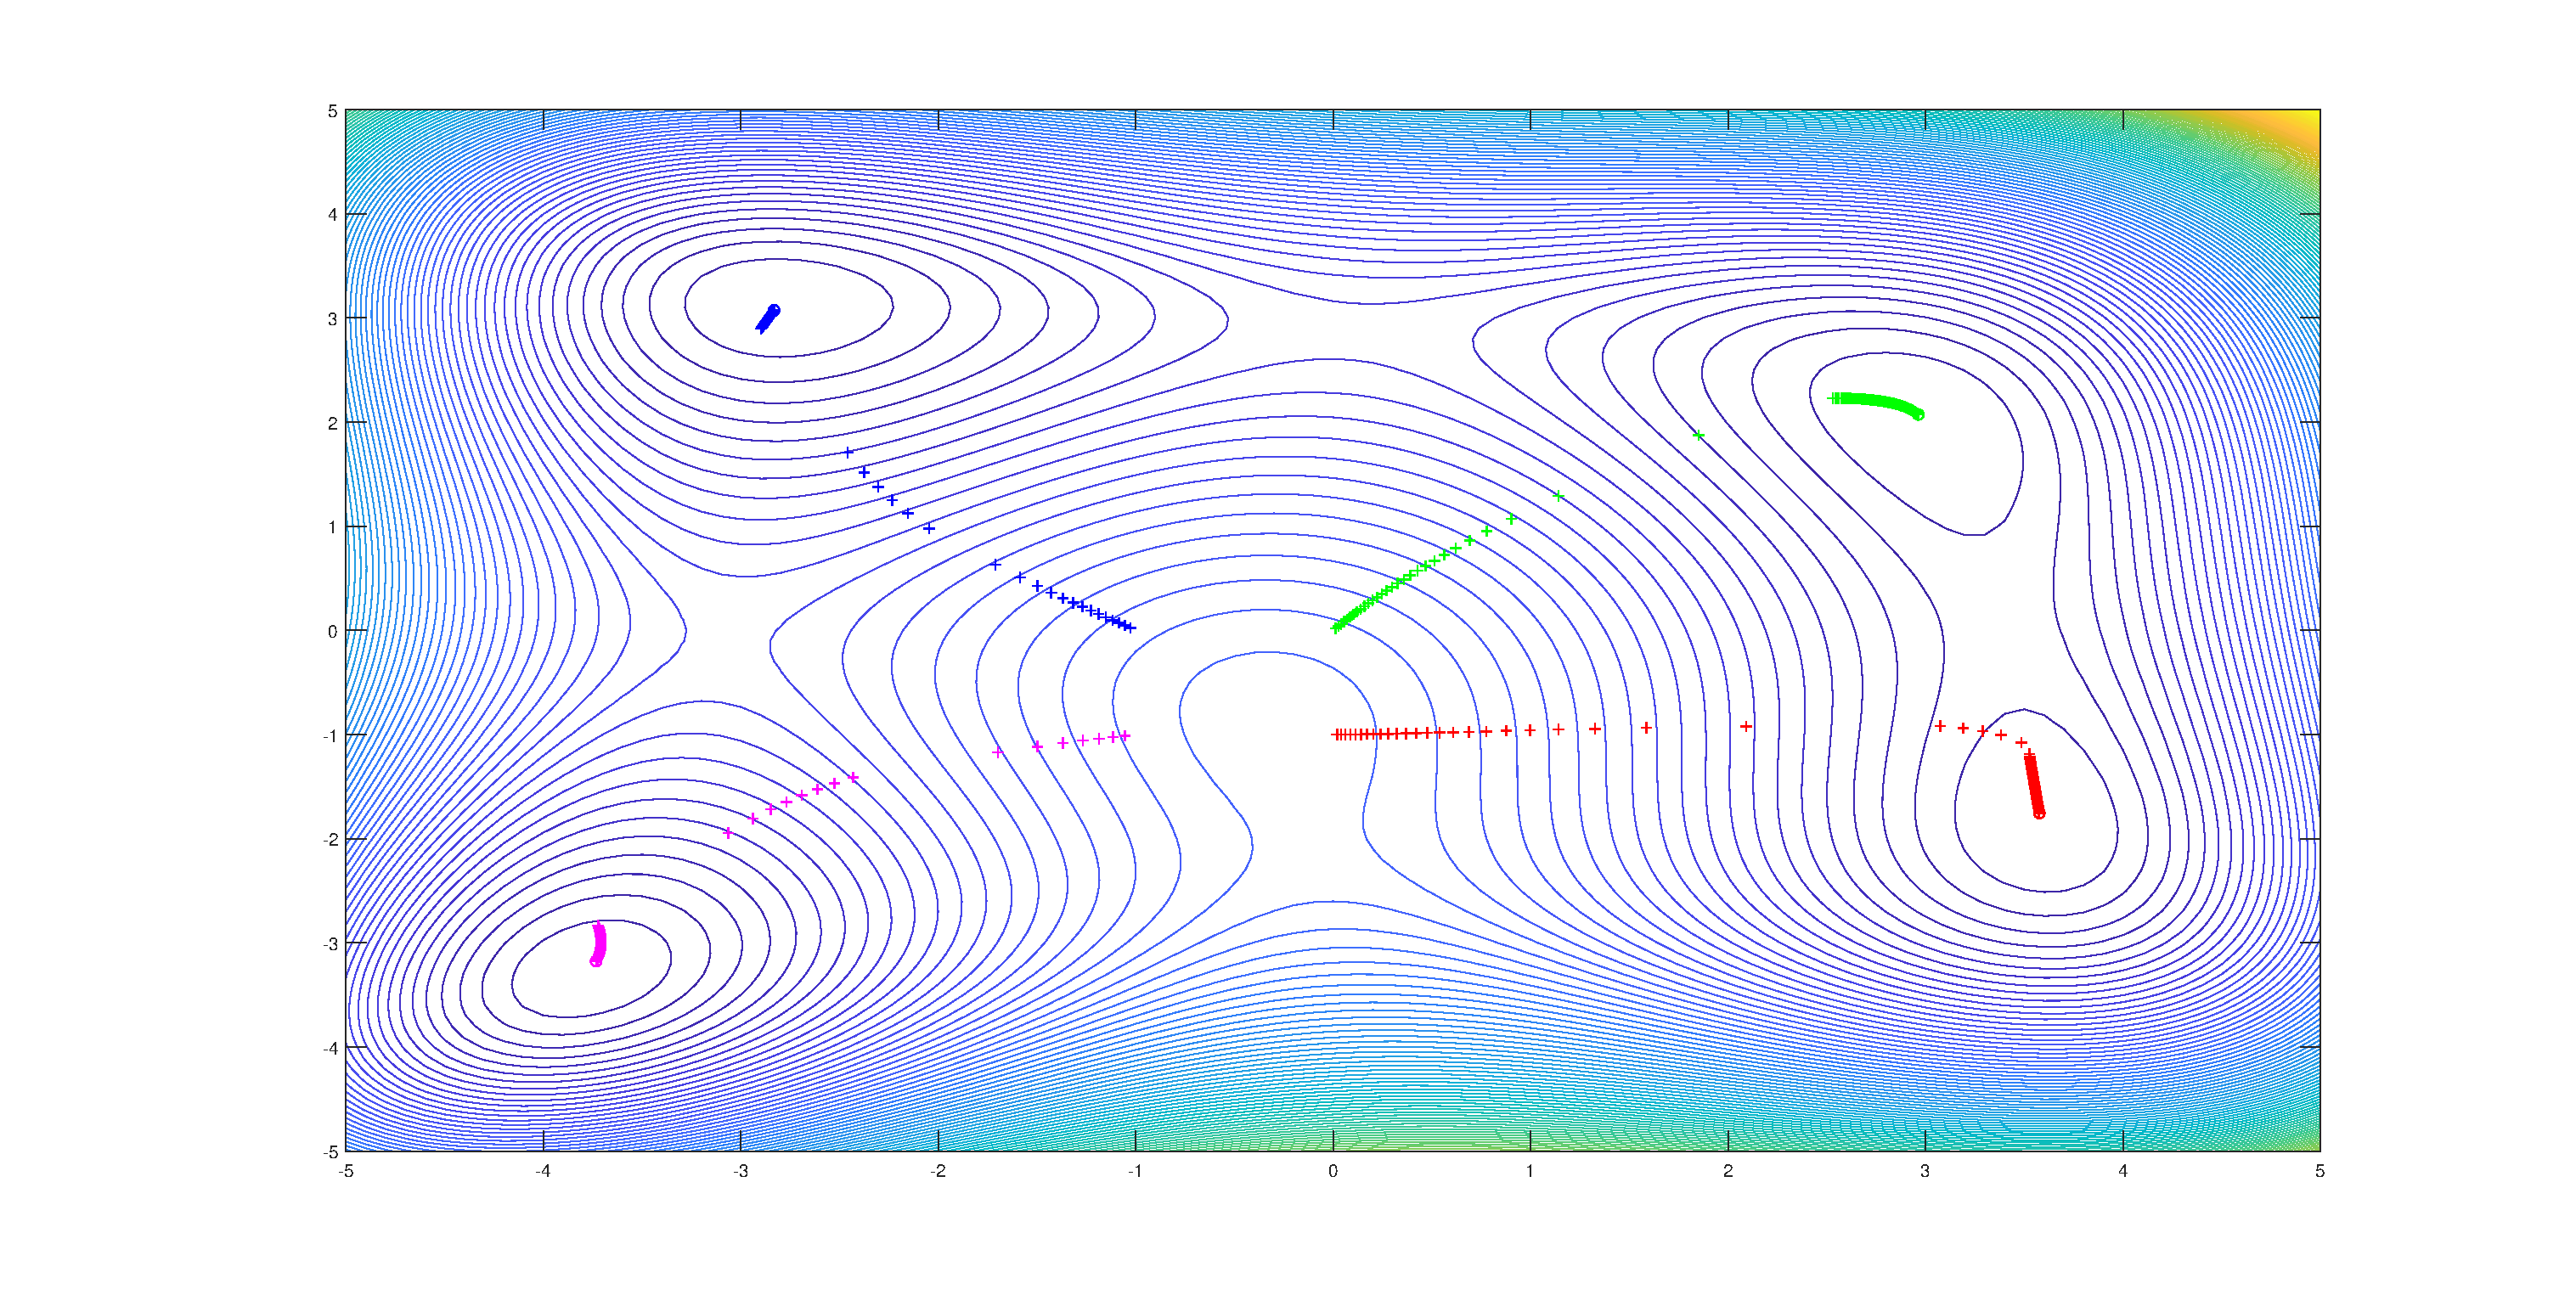
\includegraphics[width=1\textwidth]{SDM_Contour.eps}
    \caption{Caption}
    \label{fig:my_label}
\end{sidewaysfigure}
\section{Conclusion}

\pagebreak

\appendix
\section{Matlab Code}
\lstinputlisting[style=Matlab-editor, basicstyle=\mlttfamily\scriptsize, caption={Matlab Code for Solving for Force Constants}]{MSE480_Lab1.m}
\end{document}
              
            